% Book pp. 68-73 (PDF pp. 69-74)
\section{Solving Real Life Problems Involving Systems of Linear Inequalities}

Knowledge for knowledge's sake is commendable. However, utility of the
knowledge is even more satisfying. Let us go through this activity to explore the
usefulness of knowledge on solving systems of linear equations.

\begin{activity}{Activity 2.4 -- Optimising the Production of Furniture}
Working in pairs, or small groups, work on this activity.

\textbf{Scenario}

Kpogas company manufactures two types of products (chairs and tables).

Each chair requires 2 hours of carpentry and 1 hour of painting, while each
table requires 3 hours of carpentry and 2 hours of painting. The company has
a maximum of 60 hours of carpentry and 40 hours of painting available per
week.

They make a profit of \cedi50.00 per chair and \cedi80.00 per table.

How many chairs (c) and tables (t) should be produced each week to maximise
profit, while staying within the carpentry and painting constraints?

\solution
\begin{enumerate}
  \item Write out algebraic expressions for the hours of carpentry and painting.

  Hours for carpentry: $2c + 3t \le 60$

  Hours for painting: $c + 2t \le 40$
  \item Write out algebraic expressions for the number of chairs and tables.

  Number of chairs cannot be negative: c $\ge 0$

  Number of tables cannot be negative: t $\ge 0$
  \item Write out an equation for the expected profit.

  Let P represent profit

  P = 50c + 80t
  \item Express the system of linear inequalities as the constraints of production.
  \[
    \begin{cases}
      c \ge 0 \\
      t \ge 0 \\
      2c + 3t \le 60 \\
      c + 2t \le 40
    \end{cases}
  \]
  \item Note that the equation of profit is the objective function.
  \item Graph the system of linear inequalities
  \begin{center}
  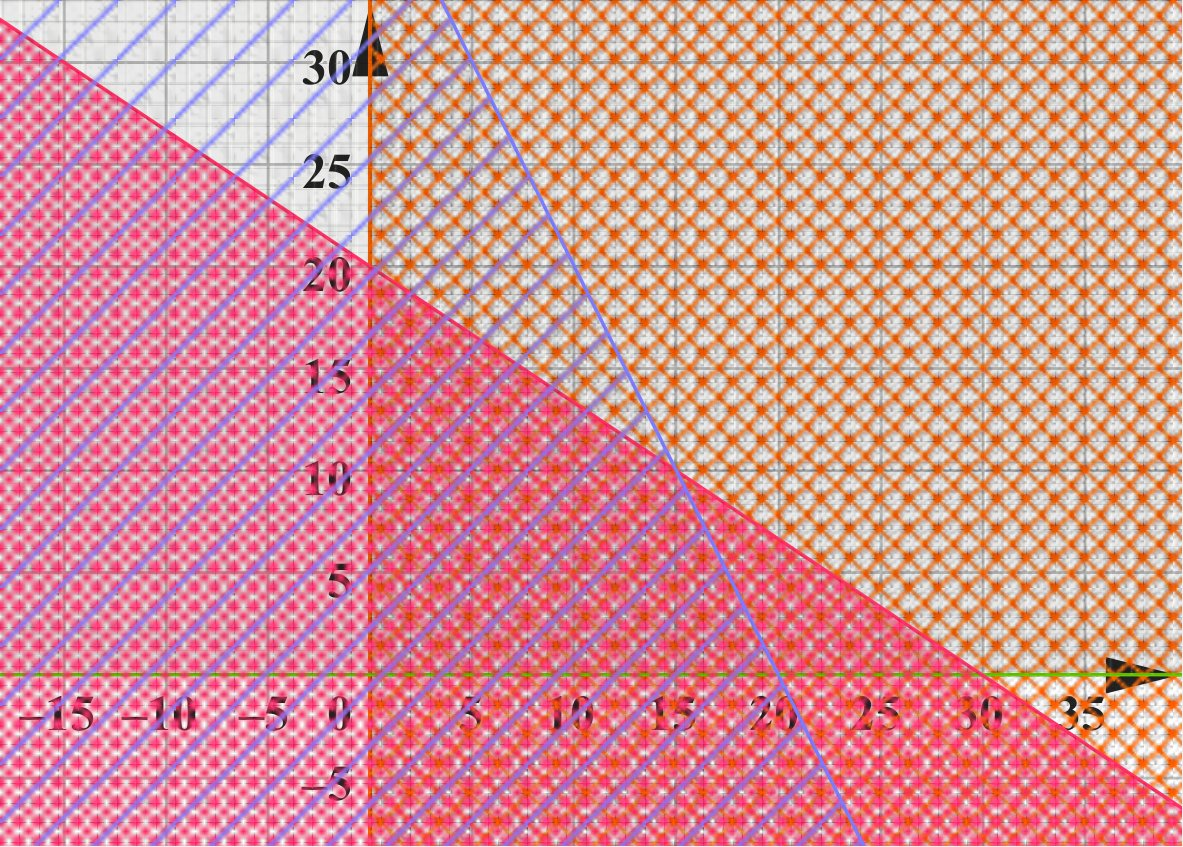
\includegraphics[width=0.85\linewidth]{figures/fig2-5.jpg}
  \end{center}
  \figcaption{2.5}{Graphical representation of Kpogas company production constraints}
  \item Identify the coordinates of the vertices to the solution region.

  $(20, 0)$, $(0, 0)$, $(15, 10)$ and $(0, 20)$
  \item Substitute the coordinates of the vertices into the profit equation.
  \begin{align*}
    \text{At } (20, 0),\ \text{P} &= 50(20) + 80(0) \\
      &= 1000 \\
    \text{At } (0, 0),\ \text{P} &= 50(0) + 80(0) \\
      &= 0 \\
    \text{At } (15, 10),\ \text{P} &= 50(15) + 80(10) \\
      &= 1550 \\
    \text{At } (0, 20),\ \text{P} &= 50(0) + 80(20) \\
      &= 1600
  \end{align*}
  \item Write out your conclusion

  The maximum profit is \cedi1600.00, and it occurs when Kpogas
  produces no chairs and 20 tables.
\end{enumerate}
\end{activity}

\begin{example}{Example 2.16}
A bakery produces cakes ($x$) and cookies ($y$) daily. A cake takes 2 hours to make
while a batch of cookies takes 1 hour to make. The bakery can spend at most 12
hours per day baking. Each cake requires 3 units of flour and a batch of cookies
requires 1 unit of flour. The bakery has at most 15 units of flour available each
day. The bakery earns \cedi5.00 profit per cake and \cedi3.00 profit per batch of
cookies. Without an increase in the units of flour and hours of baking, how many
of each product should be baked daily to make the most profit?

\solution
\textbf{Step 1:} Identify the constraints communicated by the bakery.
\[
  \begin{cases}
    2x + y \le 12 \\
    3x + y \le 15 \\
    x \ge 0 \\
    y \ge 0
  \end{cases}
\]
\textbf{Step 2:} Write out the equation of the profit (objective function).

$P = 5x + 3y$

\textbf{Step 3:} Graph the inequalities.
\begin{center}
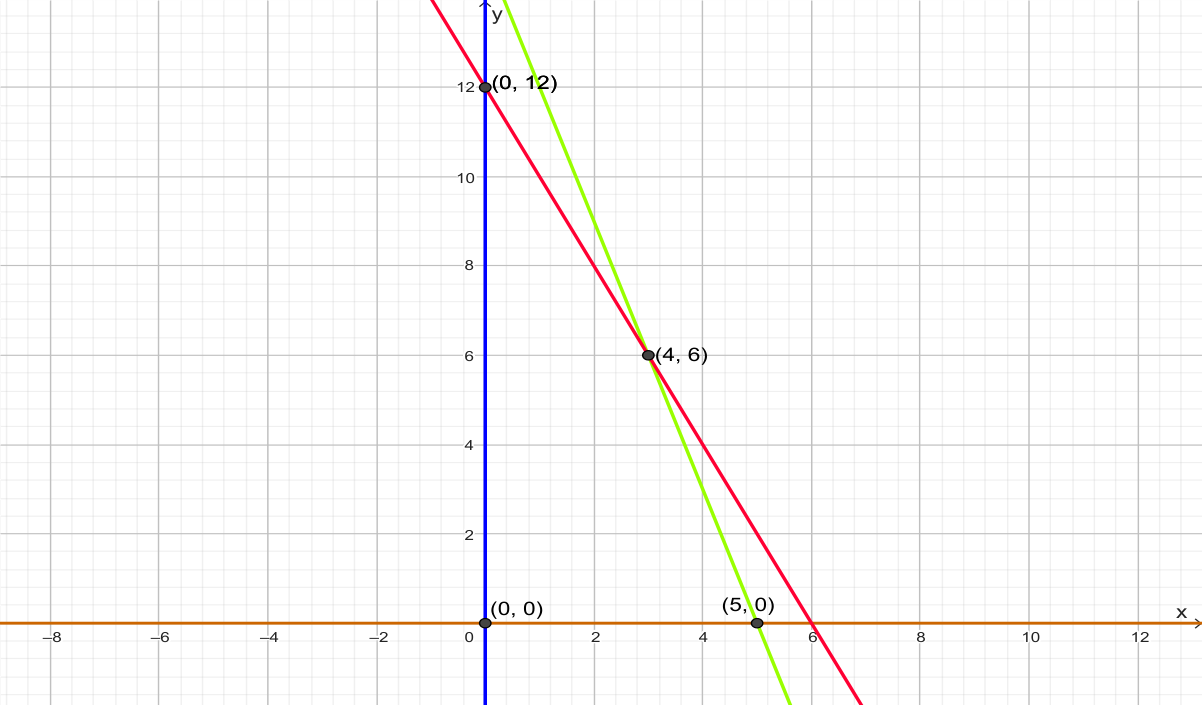
\includegraphics[width=0.85\linewidth]{figures/fig2-6.png}
\end{center}
\figcaption{2.6}{Graphical representation of constraints for baking}

\textbf{Step 4:} Identify the coordinates of the vertices to the solution region.

$(0, 12)$, $(5, 0)$, $(4, 6)$ and $(0,0)$

\textbf{Step 5:} Substitute the coordinates of the vertices into the profit equation.
\begin{align*}
  \text{At } (0, 12),\ \text{P} &= 5(0) + 3(12) \\
    &= 36 \\
  \text{At } (5, 0),\ \text{P} &= 5(5) + 3(0) \\
    &= 25 \\
  \text{At } (4, 6),\ \text{P} &= 5(4) + 3(6) \\
    &= 38 \\
  \text{At } (0, 0),\ \text{P} &= 5(0) + 3(0) \\
    &= 0
\end{align*}
\textbf{Step 6:} Write out your conclusion.

The bakery should bake 4 cakes and 6 batches of cookies daily to make the most
profit.
\end{example}

\begin{example}{Example 2.17}
A farmer has 300 metres of fencing material to enclose a rectangular field for
planting crops. The farmer wants to maximise the area of the field to get the best
crop yield, but there is a restriction. The length of the field must be 10 metres
longer than the width to accommodate the farm machinery.

What should be the dimensions of the field that will maximise the enclosed area,
keeping in mind the restriction on the total fencing available?

\solution
\textbf{Step 1:} Represent the statement algebraically.

Let w be the width of the field

Length of the field $=$ w $+\ 10$

\textbf{Step 2:} Write the equation for perimeter of the field.

Since Perimeter(P)$=$ 2(width) $+$ 2(length),
\begin{align*}
  \text{P} &= 2\text{w} + 2(\text{w} + 10) \\
  \text{P} &= 2\text{w} + 2\text{w} + 20 \\
  \text{P} &= 4\text{w} + 20.
\end{align*}
\textbf{Step 3:} Set up the linear inequality

Since the material available for fencing is 300m, the total distance around the
field can be less or equal to 300.

$4\text{w} + 20 \le 300$

\textbf{Step 4:} Simplify the inequality.
\begin{align*}
  4\text{w} &\le 300 - 20 \\
  4\text{w} &\le 280 \\
  \text{w} &\le \frac{280}{4} \\
  \text{w} &\le 70
\end{align*}
So, the width of the field must be less than or equal to 70 metres.

\textbf{Step 5:} Test values for width.

Since the highest value for the width will be 70, the length will be $70 + 10 = 80$

Testing for perimeter, $2(70) + 2(80) = 300$, satisfying perimeter requirement.

Testing for maximum area of the rectangular field: length $\times$ width

Area $= 70 \times 80 = 5600m^2$

\textbf{Step 6:} State your conclusion

The area can be maximised when the rectangle has dimensions of 70 by 80,
satisfying all constraints.
\end{example}

\begin{activity}{Activity 2.5 -- Real Life Project Involving Linear Inequalities}
\begin{enumerate}
  \item Identify an industry or company that produces/manufactures goods in
  your locality.
  \item Obtain the restrictions/constraints guiding the production of their goods.
  \item Identify the profit made on the items of production.
  \item Write a two-page report comprising:
  \begin{enumerate}
    \item[a.] where the company is located.
    \item[b.] goods produced and constraints communicated by the company
    officials.
    \item[c.] expected profit on each of the goods.
    \item[d.] an algebraic representation of constraints and objective function.
    \item[e.] a graphical representation of constraints (manually or by software).
    \item[f.] a suggestion on the decision the company should make to minimise
    profit.
    \item[g.] a suggestion on the decision the company should make to maximise
    profit.
    \item[h.] conclusion based on your observations and findings.
  \end{enumerate}
\end{enumerate}
\end{activity}
